% Suggested filename: מדריך_מהיר_לניקוי_נתוני_גלישה.tex
\documentclass[12pt]{article}

%========== (1) Math Packages ==========
\usepackage{amsmath,amssymb,amsthm}

%========== (2) General Packages: Hebrew support, fonts, etc ==========
\usepackage{xcolor}
\usepackage{float}
\usepackage{graphicx}
\usepackage{hyperref}
\usepackage{booktabs}
\usepackage{enumerate}
\usepackage{fancyvrb}
\usepackage{fancyhdr}
\usepackage{setspace}
\usepackage[most]{tcolorbox}

% Font and Language packages must come after tcolorbox for XeLaTeX/LuaLaTeX
\usepackage{fontspec}
\usepackage{polyglossia}

% Hyperref link color settings (Moved here as per typical requirements after graphicx but before language)
% Setting links to black/invisible is cleaner for documents meant for print or non-interactive PDF
\hypersetup{
  colorlinks=true,
  linkcolor=black,
  urlcolor=black,
  citecolor=black
}

% Language settings
\setdefaultlanguage{hebrew}
\setotherlanguage{english}

% Fonts
% David CLM is a standard Hebrew font. Times New Roman for English.
\newfontfamily\hebrewfont[Script=Hebrew]{David CLM}
\newfontfamily\englishfont{Times New Roman}
% Assuming David CLM is suitable for tt font as well, or specify a different Hebrew monospace font if available/preferred.
\newfontfamily\hebrewfonttt[Script=Hebrew]{David CLM} 


% Quotes - polyglossia provides \enquote{}
% \newcommand{\enquote}[1]{\textquotedblleft #1\textquotedblright}


%========== Spacing and Paragraphs ==========
% 1.5 line spacing
\onehalfspacing
% Space between paragraphs
\setlength{\parskip}{6pt}
% No paragraph indentation
\setlength{\parindent}{0pt}

%========== Header/Footer Settings ==========
% Using the later specified simple setup
\pagestyle{fancy}
\setlength{\headheight}{14.5pt} % Recommended size, adjust if warnings appear
\addtolength{\topmargin}{-2.5pt} % Small adjustment often needed with fancyhdr
\fancyhf{} % Clear header and footer
\lhead{} % Empty left header
\rhead{\today} % Date on the right header
\cfoot{\thepage} % Page number in the center footer
\renewcommand{\headrulewidth}{0pt} % No rule line for header
\renewcommand{\footrulewidth}{0pt} % No rule line for footer


%========== tcolorbox Setup ==========
% General tcolorbox setup - specific boxes override this
% Using slightly more saturated but soft colors as requested
\tcbset{
  colback=blue!5!white,        % Soft blue background
  colframe=blue!50!black,       % Stronger blue frame
  fonttitle=\bfseries,          % Bold title
  boxsep=5pt,                   % Space outside the box boundary
  top=5pt, bottom=5pt, left=5pt, right=5pt, % Internal padding
  %middle=5pt % 'middle' is for separating title from content, maybe not needed here
}

%========== Special Boxes: Definition, Remark, Example ==========
% Colors adjusted for a slightly darker, less pale look as requested
\newtcolorbox{definitionBox}[1]{
  title=#1,
  colback=green!15!white,       % Slightly darker green background
  colframe=green!70!black,      % Stronger green frame
  sharp corners,                % No rounded corners (as per example)
  enhanced,                     % Required for some features like sharp corners
  % If rounded corners desired, use 'rounded corners' instead of 'sharp corners'
}

\newtcolorbox{remarkBox}[1]{
  title=#1,
  colback=orange!15!white,      % Slightly darker orange background (nicer than yellow?)
  colframe=orange!70!black,     % Stronger orange frame
  sharp corners,
  enhanced
}

\newtcolorbox{exampleBox}[1]{
  title=#1,
  colback=red!15!white,         % Slightly darker red background
  colframe=red!70!black,        % Stronger red frame
  sharp corners,
  enhanced
}

% Bullet fix for Hebrew lists
\renewcommand{\labelitemi}{$\bullet$} % Using a proper bullet symbol

% ToC setup - keep as requested even if no ToC is used in this specific document
\usepackage{tocloft}
\usepackage{etoolbox}
\makeatletter
\renewcommand\tableofcontents{\section*{ \contentsname}
    @starttoc{toc}}
\makeatother


\begin{document}

%========== Document Title ==========
\section*{מדריך מהיר לפתרון בעיות גישה בלמדה}
% No table of contents requested or needed for this short guide.

%========== מבוא (Introduction) ==========
\section*{מבוא}

נתקלתם בבעיה בכניסה או בתצוגה של תכנים במערכת הלמידה ('למדה')? לעיתים, הבעיה נובעת מנתוני גלישה ישנים השמורים בדפדפן. \textbf{חשוב להדגיש שמדובר בבעיה זמנית} והפתרון לרוב פשוט ומהיר. המדריך הבא ילווה אתכם צעד אחר צעד בתהליך ניקוי הנתונים בדפדפנים הנפוצים.

%========== חלק 1: כרום במחשב ==========
\section*{חלק 1: ניקוי נתונים בדפדפן כרום (Chrome) במחשב}

% Include Image for Chrome PC
\begin{figure}[H]
  \centering
  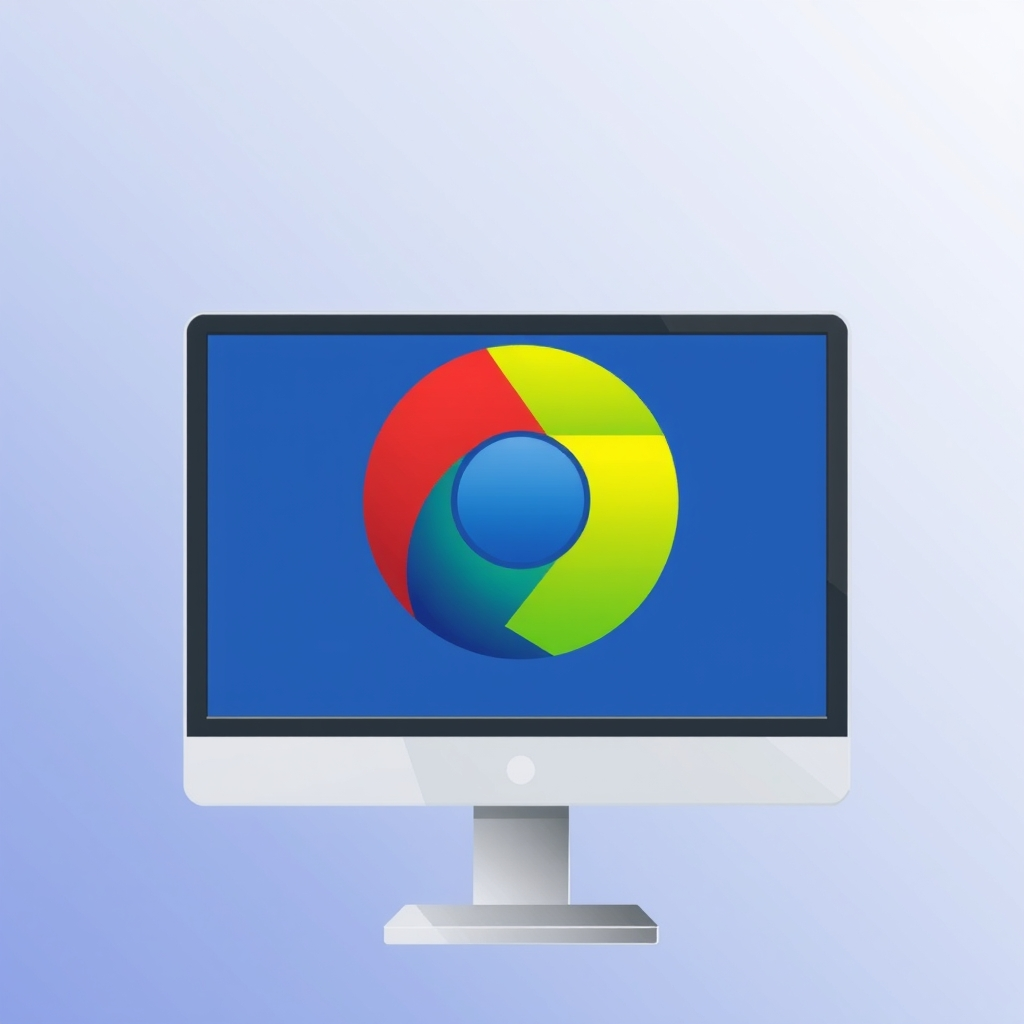
\includegraphics[width=0.4\textwidth]{files/chrome_pc_icon.png}
  \caption{אייקון דפדפן כרום בסביבת עבודה של מחשב.}
\end{figure}

מדריך זה מסביר כיצד לנקות את נתוני הגלישה בדפדפן גוגל כרום כאשר אתם משתמשים במחשב (Windows, macOS, Linux).

\begin{enumerate}
    \item פתחו את דפדפן כרום.
    \item לחצו על סמל שלוש הנקודות (\(\vdots\)) בפינה השמאלית העליונה של החלון.
    \item בתפריט שנפתח, נווטו אל \enquote{היסטוריה} ולאחר מכן לחצו שוב על \enquote{היסטוריה}. (ניתן להשתמש בקיצור המקלדת: \texttt{Ctrl+H}).
    \item בחלון ההיסטוריה, לחצו על \enquote{ניקוי נתוני גלישה} בתפריט הצדדי.
    \item בחלון הקופץ, תחת \enquote{טווח זמן}, בחרו באפשרות \enquote{כל הזמנים} (All time).
    \item ודאו שהאפשרויות הבאות מסומנות ב-V:
    \begin{itemize}
        \item \enquote{היסטוריית גלישה} (Browsing history)
        \item \enquote{קובצי Cookie ונתוני אתרים אחרים} (Cookies and other site data)
        \item \enquote{תמונות וקבצים שמורים במטמון} (Cached images and files)
    \end{itemize}
    \item לסיום, לחצו על הכפתור הכחול \enquote{ניקוי נתונים}.
\end{enumerate}

%========== חלק 2: כרום באנדרואיד ==========
\section*{חלק 2: ניקוי נתונים בדפדפן כרום (Chrome) באנדרואיד}

% Include Image for Chrome Android
\begin{figure}[H]
  \centering
  
\includegraphics[width=0.3\textwidth]{files/chrome_android_icon.png}
  \caption{אייקון אפליקציית כרום במכשיר אנדרואיד.}
\end{figure}

אם אתם משתמשים במערכת הלמידה דרך הטלפון הנייד עם מערכת הפעלה אנדרואיד, בצעו את השלבים הבאים לניקוי נתונים באפליקציית כרום:

\begin{enumerate}
    \item פתחו את אפליקציית כרום בטלפון.
    \item לחצו על סמל שלוש הנקודות (\(\vdots\)) בפינה העליונה.
    \item לחצו על \enquote{היסטוריה}.
    \item לחצו על \enquote{נקה נתוני גלישה...}.
    \item ודאו שאתם בלשונית \enquote{מתקדם}, ובחרו \enquote{כל הזמנים} בטווח הזמן.
    \item סמנו את אותן שלוש האפשרויות מהמדריך למחשב:
    \begin{itemize}
        \item \enquote{היסטוריית גלישה}
        \item \enquote{קובצי Cookie ונתוני אתרים אחרים}
        \item \enquote{תמונות וקבצים שמורים במטמון}
    \end{itemize}
    \item לחצו על \enquote{נקה נתונים}.
\end{enumerate}

%========== חלק 3: ספארי באייפון ==========
\section*{חלק 3: ניקוי נתונים בדפדפן ספארי (Safari) באייפון}

% Include Image for Safari iPhone
\begin{figure}[H]
  \centering
  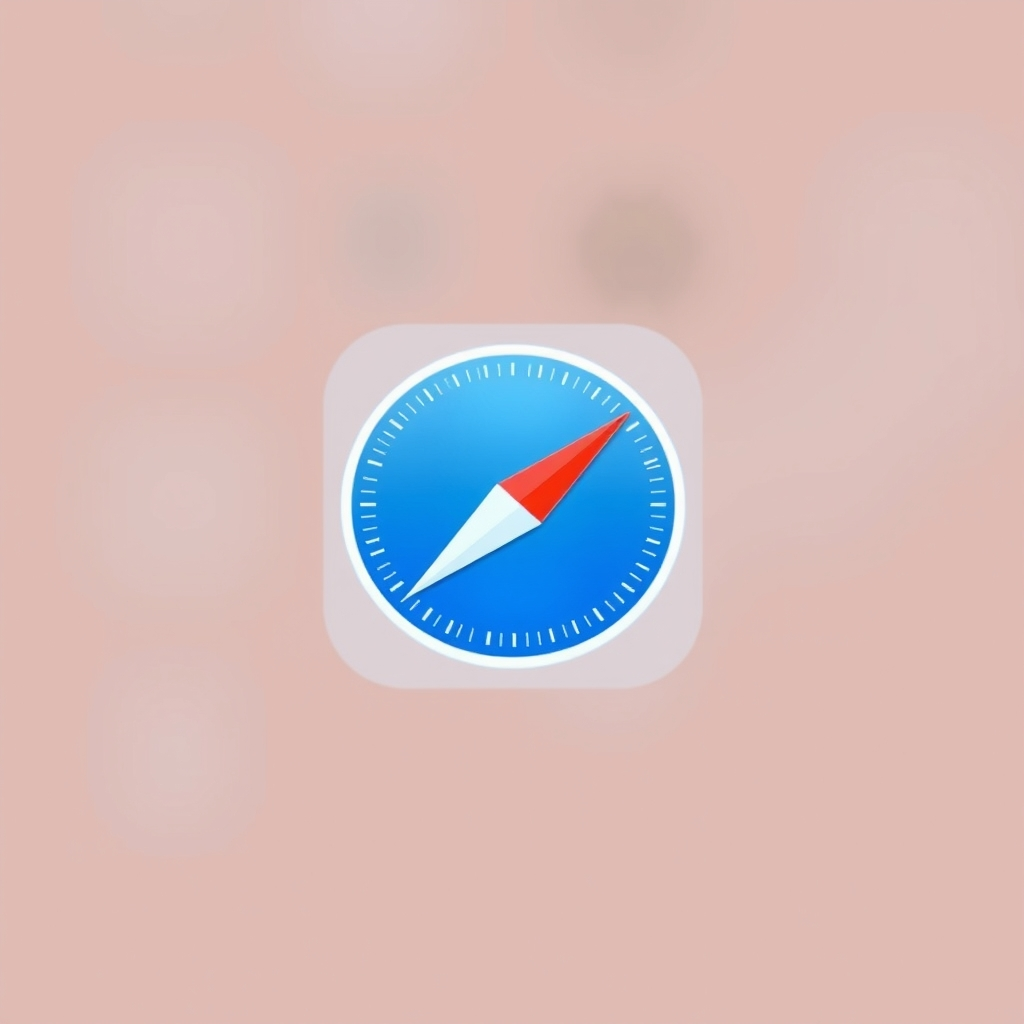
\includegraphics[width=0.35\textwidth]{files/safari_iphone_icon.png}
  \caption{אייקון דפדפן ספארי במכשיר אייפון.}
\end{figure}

למשתמשי אייפון המשתמשים בדפדפן ספארי, תהליך ניקוי הנתונים מתבצע דרך הגדרות המכשיר:

\begin{enumerate}
    \item פתחו את אפליקציית \enquote{הגדרות} במכשיר האייפון.
    \item גללו מטה ומצאו את \enquote{Safari}, ולחצו עליה.
    \item גללו מטה ולחצו על האפשרות \enquote{נקה היסטוריה ונתוני אתרים}.
    \item בחלון האישור, לחצו שוב על \enquote{נקה היסטוריה ונתונים}.
\end{enumerate}

% Use a remark box for the important note about Safari
\begin{remarkBox}{הערה חשובה למשתמשי ספארי באייפון:}
פעולה זו מוחקת את כל היסטוריית הגלישה, קובצי ה-Cookie ונתונים נוספים השמורים בספארי. שימו לב שפעולה זו \textbf{עלולה לנתק אתכם מאתרים שהתחברתם אליהם} (כמו למשל, אתר הבנק, רשתות חברתיות וכו') ותצטרכו להתחבר אליהם מחדש.
\end{remarkBox}


%========== סיכום (Summary) ==========
\section*{סיכום}

לאחר ביצוע הפעולות המתוארות במדריך, סגרו ופתחו מחדש את הדפדפן (במחשב או בטלפון, בהתאם למכשיר בו ביצעתם את הניקוי) ונסו לגשת שוב למערכת הלמידה. ברוב המקרים, ניקוי נתוני הגלישה יפתור את בעיות הגישה או התצוגה שנתקלתם בהן. בהצלחה!

\end{document}